\chapter{Research Prototype}
\label{chapter:prototype}
The above outlined key concepts were then developed into the key features of our research prototype, \textit{AmbientTeams}. Before stepping into the core features employed in AmbientTeams and aligning them to the above-mentioned key concepts (see \autoref{chapter:approach}), a brief introduction into the more technical aspects and a general overview of the application are given.

\section{Architecture}
AmbientTeams is a cross-platform desktop application based on Electron\footnote{\url{https://www.electronjs.org/}}. To facilitate the implementation of the interactive user interface in AmbientTeams, VueJS\footnote{\url{https://vuejs.org/}} is used as the JavaScript framework for the front-end. To maintain JavaScript as a common language for the front-end and back-end, NodeJS\footnote{\url{https://nodejs.org/}} is used on the server-side. The server provides both a REST API for basic CRUD functionality for users and teams and a WebSocket endpoint since much of the data required for AmbientTeams comes from the server in real-time.

\section{Teams and \enquote{Favorites}}
There are two types of teams in AmbientTeams; regular teams are stored on the server and require a unique identifier to join, similar to a straightforward invite-based approach often seen in practice. For scenarios where a user is part of multiple such teams, team members from different teams can be linked to a \enquote{favorites} team. These favorite teams only exist on the local machines of the users. In general, there is no visual difference between the two types within AmbientTeams, except that 1) there is no always-on breakroom for Favorite Teams, and 2) team members of a Favorite Team combine all status and direct messages when a Favorite Team member is part of multiple regular teams. This is different from regular teams, where status messages and direct messages are limited to that one team.

\section{Avatars}
At the core of our approach are the avatar representations of the users. While we could have opted for traditional profile pictures that allow users to upload an actual photograph, we decided to use the abstract form due to privacy reasons, and additionally allowing relatively simple mood manipulation on such avatars. Also, using an avatar library gives the user interface a more clean, uniform look, which is why we make use of getavataaars\footnote{\url{https://getavataaars.com}} to create and manipulate avatars. Users are asked to create their own avatar during the sign-up process and have the possibility to change the appearance later on. To represent the currently selected mood of each user, AmbientTeams automatically adjusts the eyes, eyebrows, and mouth types supported by the getavataaars' Application Programming Interface (API) to best possibly represent the selected emoticon.

\section{Windows}
AmbientTeams consists of two main windows; the team overview and the ambient window.

\subsection{Team Overview Window}
The team overview window is responsible for maintaining a connection to the server, authenticating, login functionality, settings. Additionally, once users have authenticated inside the team overview window, they are redirected to the team overview view where all teams and team members are visible (see \autoref{fig:at_overview}). By clicking on the edit icon next to the team name, the user can select team members from each team that will then be displayed on the other main window, the ambient window. This is demonstrated in \autoref{fig:at_overview}, where the user is selecting the team members to be displayed on the ambient window. In summary, apart from authentication purposes and initial application setup, the team overview window is primarily intended for people who are part of multiple teams and want to get a quick overview of all the different teams they belong to.

\begin{figure}[h]
    \centering
    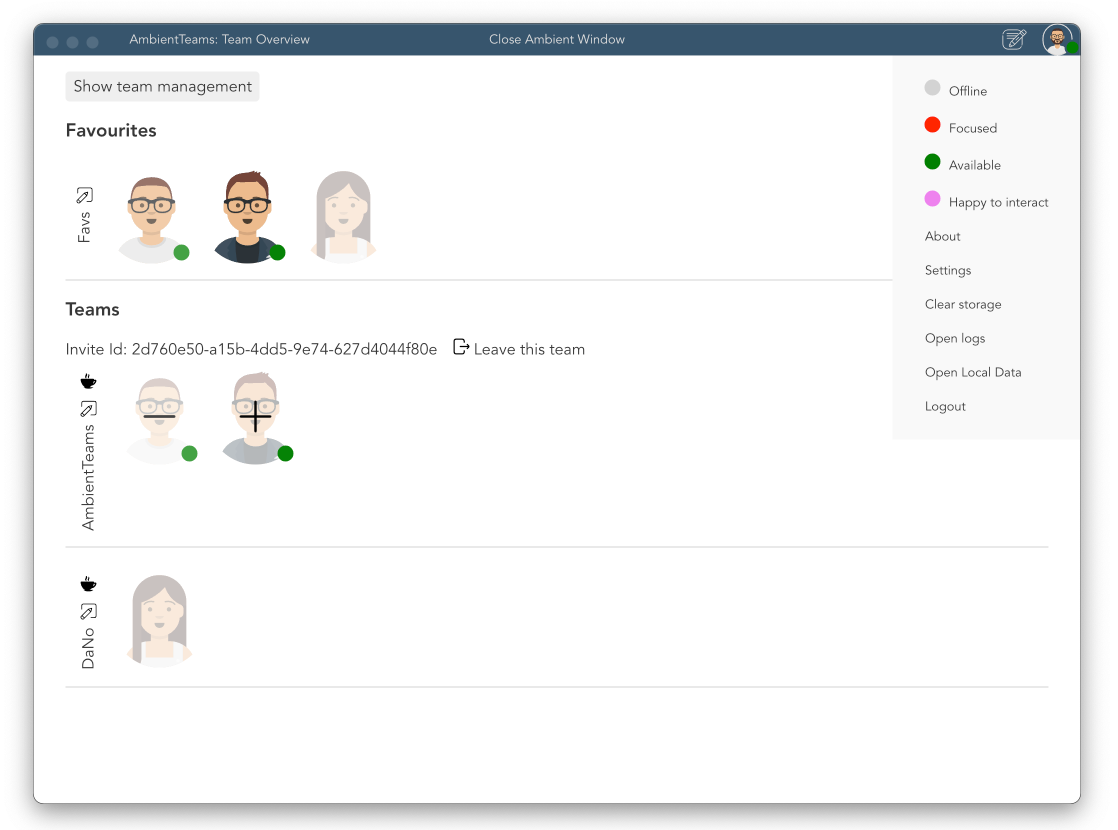
\includegraphics[width=.8\linewidth]{./images/AT_overview.png}
    \caption{Team Overview Window }
    \label{fig:at_overview}
\end{figure}

\subsection{Ambient, Glanceable Window}
The Ambient window is always on top of other windows (see \autoref{fig:at_ambient_on_top}), which on the one hand, makes it easy to stay informed about moods and other statuses of your team members, but on the other hand, can also cause interruptions and distractions. We used a transparent borderless window to keep the ambient overlay as ambient and unobtrusive as possible. However, if the window is still distracting, it can be easily minimized or closed altogether using the menu that can be accessed by clicking the minimize icon (see \autoref{fig:at_hover}). Opening the team overview window can be achieved by clicking on the three dots in the menu, which will display a small drop-down menu with the option to open the team overview window. Also, in this menu, the ambient window can be enlarged or reduced to fit different screen resolutions and personal preferences.

\begin{figure}[h]
    \centering
    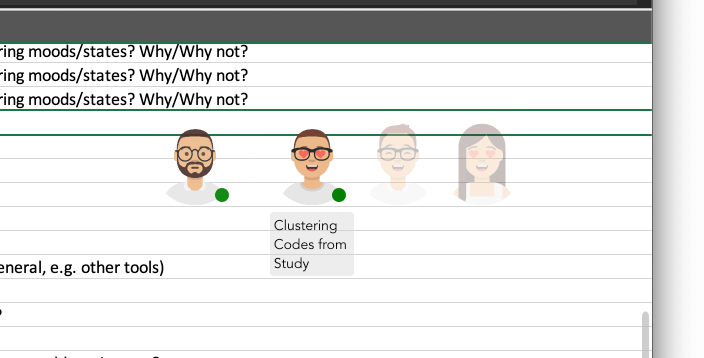
\includegraphics[width=.8\linewidth]{./images/AT_ambient_on_top.png}
    \caption{Always-on-Top Ambient Window While Working on Another Task}
    \label{fig:at_ambient_on_top}
\end{figure}

Further, certain elements are only visible when the user is hovering over this window (see \autoref{fig:hover_no_hover}). When hovering over the ambient window, the user can select the team they want to show and sees the names of the individual team members, as shown in \autoref{fig:at_hover}.

\begin{figure}[h]
    \centering
    \begin{subfigure}{.5\textwidth}
        \centering
        
\includegraphics[width=.8\linewidth]{./images/AT_no_hover.png}
        \caption{No Hover}
        \label{fig:at_no_hover}
    \end{subfigure}%
    \begin{subfigure}{.5\textwidth}
        \centering
        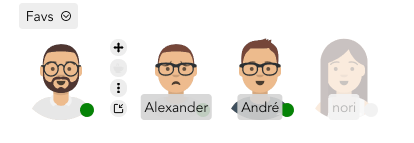
\includegraphics[width=.8\linewidth]{./images/AT_hover.png}
        \caption{Hover}
        \label{fig:at_hover}
    \end{subfigure}
    \caption{Ambient Window}
    \label{fig:hover_no_hover}
\end{figure}

\section{Availability Status}
AmbientTeams wants to keep the number of interruptions to a minimum, which is why there is the \enquote{Focused} availability state (see \autoref{fig:call}) that exists in addition to the three others (\enquote{Available}, \enquote{Offline}, and \enquote{Happy to Interact}). Users in this focused state cannot be called. Further, they don't see any direct messages or incoming nudges until they leave the focused state. In addition, focused users cannot directly interact with other team members, avoiding potential self-distraction. The availability state \enquote{Happy to Interact} was included to address the lack of serendipity in remote work. When selected by at least two team members, an automatic matchmaker runs every minute and randomly pairs two people, who are then routed to a video call.

\section{Sharing Moods and Status Messages}
The user can open the sharing window from both the team overview and the ambient window, and the system tray menu. All of those actions will open the sharing window as shown in \autoref{fig:sharing_manual}, where on the left, a preview of the current avatar and the selection of available moods are listed. There are nine available moods, visualized using popular emoticons available through OpenMoji\footnote{\url{https://openmoji.org}}, an open-source emoji project. The first four of the available emoticons are more optimistic, the fifth is a neutral face, and the last four are emoticons representing rather negative emotional states. The selection of the emoticons started with six basic emotions: surprise, fear, disgust, anger, happiness, and sadness \autocite{an2017two}. This list was expanded over time to better suit the work environment by adding a neutral and tired emoticon and two more positive emotions (loving hearts and grinning) to make the selection more balanced. Due to limitations with the avatar API, we could not render \enquote{fear} well enough, which led us to remove it. On the right, the user can enter additional context in a simple, standard textbox. The contents of this textbox are, if available, pre-populated with the current status message for the currently selected team. Additionally, the text is highlighted when the window is created, facilitating overwriting the current status without using the mouse to select the text manually. The status messages' length is limited to 140 characters, motivated by the initial limit of Twitter \autocite{dullemond2013fixing}. Below the textbox, the user can find a button to share the status message with either all teams or a single team.

As a reminder for the user to share their moods and potential additional context with team members, the sharing window also appears automatically at pre-defined times. The location we chose for this popup is the lower right corner of the user's primary monitor to minimize the potential for distraction. Overall, the window has the same functionality but includes two additional buttons to defer the prompt for either 5 minutes or 1 hour (see \autoref{fig:sharing_auto}). The scheduled sharing window is displayed at three pre-defined times throughout the day, namely at 9:00, 13:00, and 16:00 local time. We chose those times because that is when most people are already or will still be working.

\begin{figure}[h]
    \centering
    \begin{subfigure}{.5\textwidth}
        \centering
        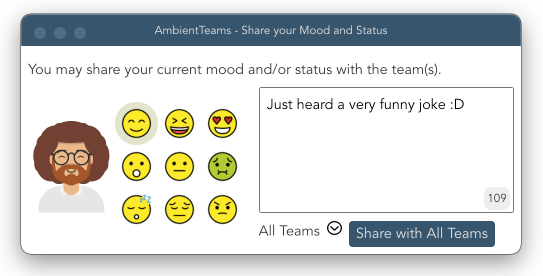
\includegraphics[width=.8\linewidth]{./images/sharing_manual.png}
        \caption{Manually Opened}
        \label{fig:sharing_manual}
    \end{subfigure}%
    \begin{subfigure}{.5\textwidth}
        \centering
        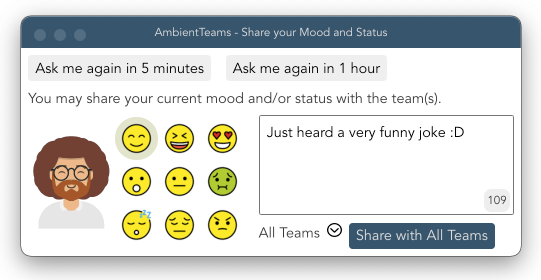
\includegraphics[width=.8\linewidth]{./images/sharing_auto.png}
        \caption{Scheduled}
        \label{fig:sharing_auto}
    \end{subfigure}
    \caption{Sharing Window}
\end{figure}

To ensure that the information shared within AmbientTeams is always up-to-date, a few measures have been taken. The first is purely visual: avatars are increasingly hidden the longer there has been no current activity. Such activities include status and mood sharing, direct messaging, and nudging. This automatic hiding should motivate users to interact with such hidden team members and easily spot updates from colleagues. Another measure we have taken to avoid showing users outdated content is automatically resetting status updates and moods at midnight.

Since the goal of AmbientTeams is to encourage informal communication, there is no chat history or other history built into the application. With this feature, we want to promote more casual and less formal communication and hope to avoid AmbientTeams becoming just another tool to keep track of.

\section{Ever-Running Breakroom}
As mentioned before, our goal was to create ever-running breakrooms as effortlessly as possible. \autoref{fig:breakroom_initiator} shows the state of the ambient window when the user has clicked on the coffee icon. After the user clicks on this coffee icon, the other team members will see an indication that there is a breakroom in progress (see \autoref{fig:breakroom_indicator}). However, to avoid unnecessarily creating a breakroom and potentially interrupting the initiating user, the breakroom is not created until another user clicks on the coffee icon.

\begin{figure}[h]
    \centering
    \begin{subfigure}{.5\textwidth}
        \centering
        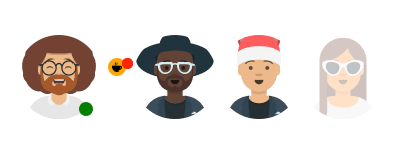
\includegraphics[width=.8\linewidth]{./images/breakroom_initiator.png}
        \caption{Initiating a Breakroom Creation}
        \label{fig:breakroom_initiator}
    \end{subfigure}%
    \begin{subfigure}{.5\textwidth}
        \centering
        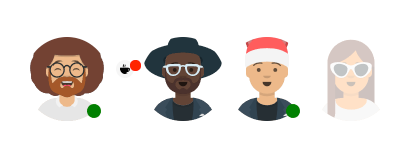
\includegraphics[width=.8\linewidth]{./images/breakroom_indicator.png}
        \caption{Joining a Breakroom }
        \label{fig:breakroom_indicator}
    \end{subfigure}
    \caption{Breakroom Creation}
\end{figure}

Once at least two team members have clicked the breakroom icon, a breakroom is created in the back-end with twilio\footnote{\url{https://www.twilio.com}}, and they are redirected to the breakroom view (see \autoref{fig:breakroom}). At any point, other team members can join and leave the breakroom, and it will remain active as long as at least one team member is present. We want to avoid users forgetting the time and staying too long in the breakroom. For this purpose, a 15-minute timer is started as soon as one enters the breakroom. When this timer reaches its end, the user automatically leaves the breakroom.

\begin{figure}[h]
    \centering
    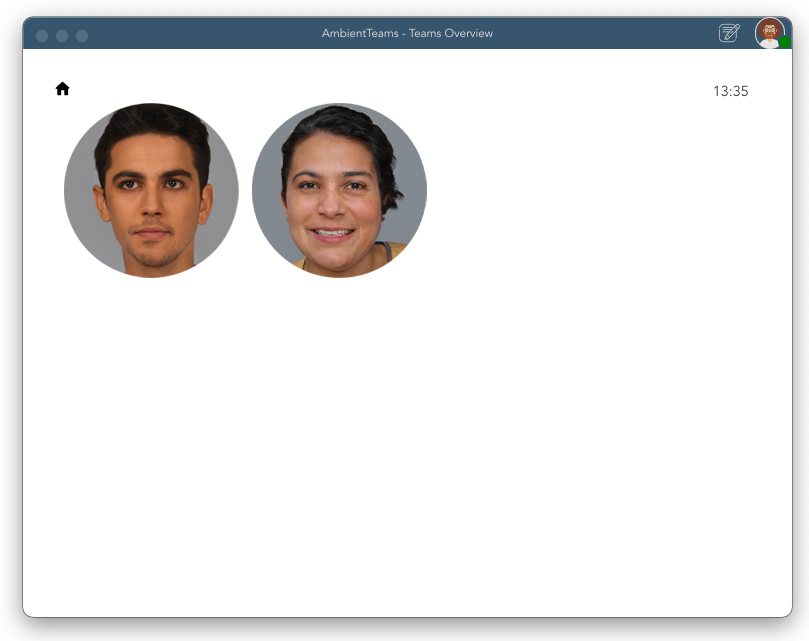
\includegraphics[width=.8\linewidth]{./images/breakroom.png}
    \caption{Ongoing Breakroom}
    \label{fig:breakroom}
\end{figure}

\section{Direct Interactions}
In addition to broadcasting moods and status messages, there is also the ability to interact directly with an individual team member. Hovering over individual team members brings up an overlay that offers three different interaction options, namely 1) direct messaging, 2) nudging, and 3) direct calling (see \autoref{fig:interactions}).

\begin{figure}[h]
    \centering
    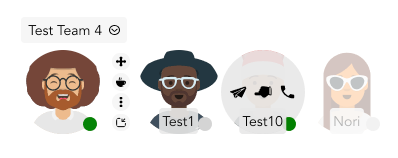
\includegraphics[width=.4\linewidth]{./images/interactions.png}
    \caption{Direct Interactions Overlay}
    \label{fig:interactions}
\end{figure}

Direct messaging is very similar to status message sharing but without mood sharing and team selection options. After clicking the message icon, the message window (\autoref{fig:messaging_window}) is displayed at the user's current mouse position to minimize the distance needed to interact with the window's contents. As in the status sharing window, there is a character limit of 140 characters.

\begin{figure}[h]
    \centering
    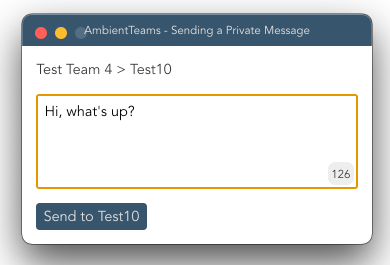
\includegraphics[width=.4\linewidth]{./images/messaging_window.png}
    \caption{Messaging Window}
    \label{fig:messaging_window}
\end{figure}

In \autoref{fig:interaction_results} all three interaction options are visualized. Direct messages (\autoref{fig:dm}) are distinguished from status messages by the message icon located to the left of the actual message. Nuding (\autoref{fig:nudging}) uses a hand icon pointing to the team member in question. For a video call (\autoref{fig:call}), the video stream overlays the team member's avatar, and the availability status of both participants is automatically set to \enquote{Focused}. Users can hover over their avatar if they want to mute or pause the video stream. To end a call, you need to hover over the corresponding team member and click the hang-up icon.

\begin{figure}[h]
    \centering
    \begin{subfigure}{.3\textwidth}
        \centering
        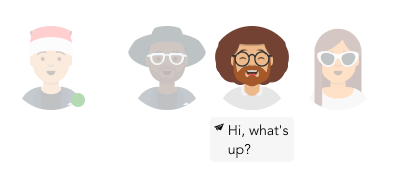
\includegraphics[width=.9\linewidth]{./images/DM.png}
        \caption{Direct Message}
        \label{fig:dm}
    \end{subfigure}%
    \begin{subfigure}{.3\textwidth}
        \centering
        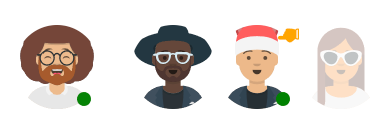
\includegraphics[width=.9\linewidth]{./images/nudging.png}
        \caption{Nudging}
        \label{fig:nudging}
    \end{subfigure}
    \begin{subfigure}{.3\textwidth}
        \centering
        
\includegraphics[width=.9\linewidth]{./images/call.png}
        \caption{Ongoing Video Call }
        \label{fig:call}
    \end{subfigure}
    \caption{Direct Interactions}
    \label{fig:interaction_results}
\end{figure}